\newlecture
\setcounter{section}{1}

%\def\textbookchapter{Chapter 10: Derivatives of Multivariable Functions}
\def\coursetopicnumber{II}
\def\topic{First-Order Partial Derivatives \& Second-Order Partial Derivatives} % this is the printed title
\def\shorttopic{First-, second-order partials} % short topic
\def\textbookname{Active Calculus} % this is the corresponding textbook
\def\shorttextbookname{AC} % this is the short name for the book
\def\textbooksection{10.2 \& 10.3} % corresponding textbook section
\def\textbooksectionurl{https://activecalculus.org/vector/S-10-2-First-Order-Partial-Derivatives.html} % URL for textbook section
\def\handoutday{} % this is the printed date

%%%%%%%%% DOCUMENT CONTENT STARTS BELOW

\thispagestyle{plain}
\topstuff
\section{First-Order Partial Derivatives \href{\textbooksectionurl}{(book link)}}
\section{Second-Order Partial Derivatives \href{https://activecalculus.org/vector/S-10-3-Second-Order-Partial-Derivatives.html}{(book link)}}
\setcounter{section}{2}

\subsection{Derivatives, graphically}
For a function $f(x)$ and an $x$ value $a$, the \emph{derivative of $f(x)$ at $x=a$} is written as $f'(a)$. We see this graphically as the slope of the tangent line to the graph of $y=f(x)$ at the point $(a,f(a))$. The value of $f'(a)$ tells us how $f(x)$ changes if we're at $x=a$ and increase $x$ a little bit.

In particular, 
\begin{itemize} 
    \item 
    if $f'(a)>0$, then if we're at $x=a$ and we increase $x$, $f(x)$ will \phantom{increase.}
    \item 
    if $f'(a)<0$, then if we're at $x=a$ and we increase $x$, $f(x)$ will \phantom{decrease.}
\end{itemize} 

\pagebreak 

\subsection{Partial derivatives via level curves}
For a function $f(x,y)$ and a point $(a,b)$, the \emph{partial derivative of $f(x,y)$ with respect to $x$ at $(x,y)=(a,b)$} is written as $f_x(a,b)$. The value of $f_x(a,b)$ tells us the rate at which $f(x,y)$ will change if we're at $(x,y)=(a,b)$ and increase $x$ a little bit.

We can interpret the partial derivatives with respect to $x$ in a manner similar to the single variable situation:
\begin{itemize}
    \item if $f_x(a,b)>0$, then if we're at $(x,y)=(a,b)$ and we increase $x$, $f(x,y)$ will \phantom{increase.}
    \item if $f_x(a,b)<0$, then if we're at $(x,y)=(a,b)$ and we increase $x$, $f(x,y)$ will \phantom{decrease.}
\end{itemize}

\bigskip 

For a function $f(x,y)$ and a point $(a,b)$, the \emph{partial derivative of $f(x,y)$ with respect to $y$ at $(x,y)=(a,b)$} is written as $f_y(a,b)$. The value of $f_y(a,b)$ tells us the rate at which $f(x,y)$ will change if we're at $(x,y)=(a,b)$ and increase $y$ a little bit.

We can interpret the partial derivatives with respect to $y$ in a manner similar to the single variable situation:
\begin{itemize}
    \item if $f_y(a,b)>0$, then if we're at $(x,y)=(a,b)$ and we increase $y$, $f(x,y)$ will \phantom{increase.}
    \item if $f_y(a,b)<0$, then if we're at $(x,y)=(a,b)$ and we increase $y$, $f(x,y)$ will \phantom{decrease.}
\end{itemize}

%As we will see in Section \ref{sec:linearization}, just as $f'(a)$ tells us about the slope of a line tangent to the graph of the curve $y=f(x)$ at $x=a$, the partial derivatives $f_x(a,b)$ and $f_y(a,b)$ tell us about slopes on a plane tangent to the graph of the surface $z=f(x,y)$ at $(x,y)=(a,b)$. 
%\pagebreak 

\begin{ex}
    Here are some level curves for $f(x,y)=\dfrac{-x^2+y}{2}.$ The marked points are $P=(-3,12)$ and $Q=(1,10)$.\\
    \mbox{} \hfill 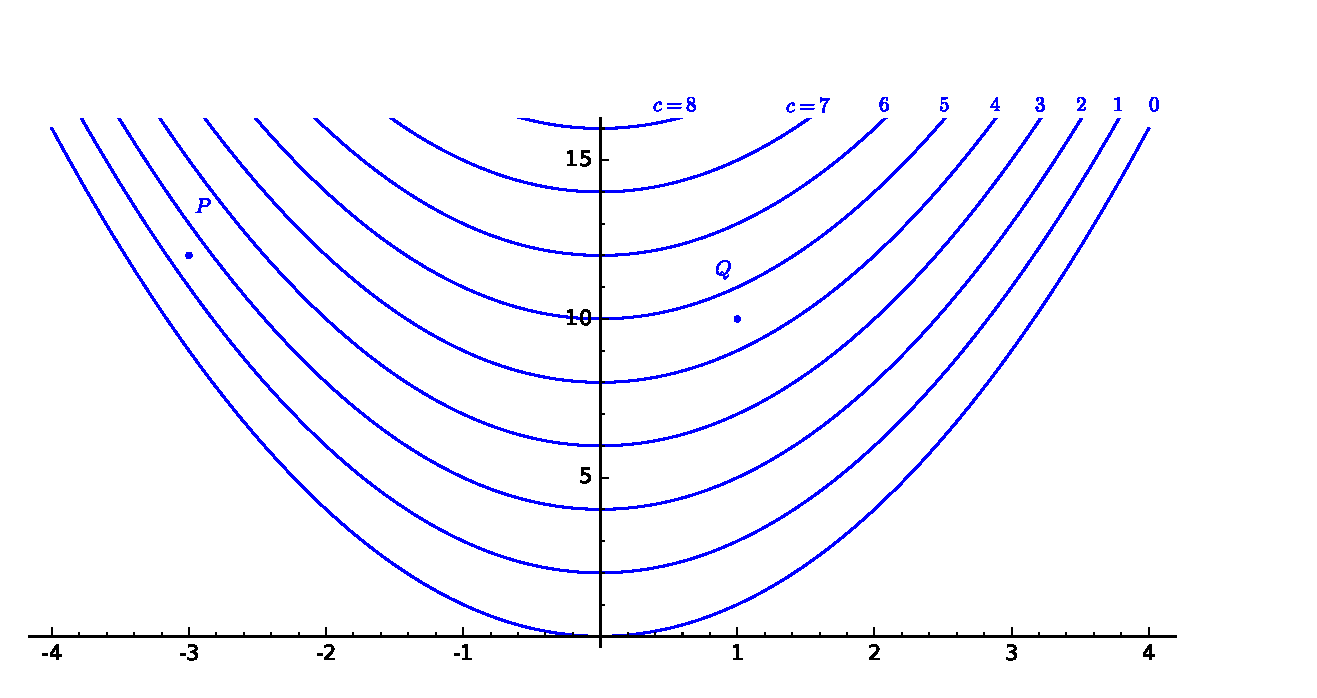
\includegraphics[width=.9\textwidth]{images/partial_deriv_intro.eps}\hfill \mbox{} \label{img:sage-level-curves}
    \\ Decide positive/negative for the following.
    \begin{multicols}{4}
    \begin{enumerate}
        \item $f_x(-3,12)$
        \item $f_y(-3,12)$
        \item $f_x(1,10)$ 
        \item $f_y(1,10)$
    \end{enumerate}
    \end{multicols}
\end{ex}

\pagebreak 



\subsection{Changes in the \texorpdfstring{$x$}{x} and \texorpdfstring{$y$}{y} directions}
\begin{ex}\label{ex:saddle-traces}
    Let $f(x,y)=x^2-y^2$. Below are two views of the graph of $z=x^2-y^2$, a hyperbolic paraboloid (saddle). Two traces are highlighted, corresponding to $y=1$ and $x=1.5$.
    \begin{center}
        \includegraphics[width=.4\textwidth]{images/saddle1.png}
        \hfill 
        \includegraphics[width=.4\textwidth]{images/saddle2.png}\label{img:sage-saddle}
    \end{center}
    Find the intersection point of the two traces. Call it $P$. Plot the traces in the $xz$- and $yz$-planes and mark $P$ on each. If you're at $P$ and increase $x$, does $f(x,y)$ increase or decrease? If you're at $P$ and increase $y$, does $f(x,y)$ increase or decrease?
\end{ex}

\pagebreak 

\subsection{Derivative notation}
In Calculus I, we defined the \emph{derivative} of $f(x)$ as $f'(x)=$ 
%\[f'(x)=\hspace{1in}\]%\lim\limits_{\Delta x\to 0}\dfrac{f(x+\Delta x)-f(x)}{\Delta x}.\]
\bigskip 

This tells us how $f(x)$ changes as we increase $x$.  

We can then take the \emph{second derivative}, $f''(x)$, which is the derivative of $f'(x)$. Whereas $f'(x)$ tells us about increasing/decreasing, $f''(x)$ tells us about bending (concavity).

And, of course, we can continue to compute derivatives, getting $f'''(x)$, $f''''(x)$, etc.
\vspace{.3in}

In general, then $n$th derivative of $f$ w.r.t.\ $x$ is denoted 
\bigskip 

%\subsection{Notation}
In addition to the prime notation $f'(x)$, we have the \emph{differential operator} $\displaystyle\dd{x}$. It basically means \begin{center}``take the derivative of the following function with respect to the variable $x$.''\end{center}  In other words, 
\[
    \dd{x}f(x) = \hide{f'(x).}
\] 
\medskip 

\noindent Note that the variable in $\dd{x}$ matches the variable in the function. This way of writing derivatives is called \emph{Leibniz notation}.
\begin{ex}
    Write the following in prime notation.
    \begin{multicols}{2}
    \begin{enumerate}
        \item $\displaystyle\dd{t} g(t)$
        \item $\displaystyle\dd{x}\left(\dd{x}f(x)\right)$
        \item $\displaystyle\frac{\dif^2 h}{\dif x^2}$
        \item $\displaystyle\left(\frac{\dif}{\dif y}\right)^2M(y)$
    \end{enumerate}
    \end{multicols}
\end{ex}
If we want to evaluate these functions, we use a vertical bar.
For a function $f(x)$, 
\[
    \left.\dd{x}f(x)\right|_{x=a}=\hide{f'(a).}
\]
Similarly, $\left.\dfrac{\dif^n}{\dif x^n}f(x)\right|_{x=a}=\phantom{f^{(n)}(a)}$
\begin{ex}
    Given $f(x)=\sin(x)+x^2$. Compute $\left.\dfrac{\dif^2}{\dif x^2}f(x)\right|_{x=\pi/2}$
\end{ex}

\pagebreak 

\subsection{Partial derivative notation \& computation}
For a function $f(x,y)$, we can investigate how it changes with respect to $x$ and how it changes with respect to $y$. These rates of change are called \emph{partial derivatives}. Just like the differential operator, we have \emph{partial derivative operators} $\dfrac{\partial}{\partial x}$ and $\dfrac{\partial}{\partial y}$.

The \emph{partial derivative of $f(x,y)$ with respect to $x$}, denoted $f_x(x,y)$ or $\dfrac{\partial}{\partial x}f(x,y)$, is defined as 
\[
    \hspace{-1in}\dfrac{\partial}{\partial x}f(x,y)=\hspace{2in}
\]
%\lim\limits_{\Delta x\to 0}\dfrac{f(x+\Delta x,y)-f(x,y)}{\Delta x}.\]

The \emph{partial derivative of $f(x,y)$ with respect to $y$}, denoted $f_y(x,y)$ or $\dfrac{\partial}{\partial y}f(x,y)$, is defined as 
\[
    \hspace{-1in}\dfrac{\partial}{\partial y}f(x,y)=\hspace{2in}
\]
%\lim\limits_{\Delta y\to 0}\dfrac{f(x,y+\Delta y)-f(x,y)}{\Delta y}.\]

The symbol $\partial$ is generally called ``partial.'' It is also often called ``del.''  Partial derivatives tell us how $f(x,y)$ is changing as we vary $x$ or $y$. \\

{\centering 
    \framebox{
        In practice, we can compute partial derivatives by treating the other variables as constants.
    }
\par}
\begin{ex}
    Let $f(x,y)=x^3-4xy^2+5xy+6$. Compute $\dfrac{\partial}{\partial x}f(x,y)$ and $\dfrac{\partial}{\partial y}f(x,y)$.
\end{ex}

\vfill\vfill

\begin{ex}
    For $f$ above, compute $\dfrac{\partial}{\partial x}\left(\dfrac{\partial}{\partial x}f(x,y)\right)$, $\dfrac{\partial}{\partial y}\left(\dfrac{\partial}{\partial x}f(x,y)\right)$, and $\dfrac{\partial}{\partial x}\left(\dfrac{\partial}{\partial y}f(x,y)\right)$.
    %$\left.\dfrac{\partial}{\partial x}\left(\dfrac{\partial}{\partial y}f(x,y)\right)\right|_{(x,y)=(1,2)}$
\end{ex}

\vfill\vfill\vfill

\pagebreak
%\subsection{Shortcut notation}

We write $f_x(x,y)=\dfrac{\partial}{\partial x}f(x,y)$ and $f_y(x,y)=\dfrac{\partial}{\partial y}f(x,y)$.

We can mimic higher-order derivatives too. If we want to take a partial derivative of $f(x,y)$ with respect to $x$ and then take the partial derivative of that with respect to $y$, we can write that as $f_{xy}(x,y)$.

\vspace{1.5in}

\begin{ex}
    Let $g(x,y)=x(2x+3y)^4+5$. Compute $g_{xx}(x,y)$, $g_{xy}(x,y)$, and $g_{yx}(x,y)$. %, and $g_{yy}(x,y)$. 
    %Then evaluate $\left.\dfrac{\partial^2}{\partial x\partial y}g(x,y)\right|_{(x,y)=(1,\pi)}$
\end{ex}

\vfill 

\begin{thm}[Clairaut's Theorem]
    Let $f$ be a function of more than one variable for which the partial derivatives $f_{xy}$ and $f_{yx}$ are continuous near the point $(a,b)$. Then
    \[
        f_{xy}(a,b) = f_{yx}(a,b).
    \]
\end{thm}

\vspace{1in}

\pagebreak 

\subsection{Computation and interpretation}
\begin{ex}
    Let $f(x,y)=x^2-y^2$. Compute $f_x(1.5,1)$, $f_y(1.5,1)$, $f_{xx}(1.5,1)$, and $f_{yy}(1.5,1)$. How do these relate to Exercise~\ref{ex:saddle-traces}?
\end{ex}

\vfill

\begin{ex}
    Let $f(x,y)=x^3-x^2y+xy^4$. At $(x,y)=(1,-2)$,
    \begin{enumerate}
        \item is $f(x,y)$ increasing or decreasing if we increase $x$ a bit?
        \item is $f(x,y)$ increasing or decreasing if we increase $y$ a bit?
    \end{enumerate}
\end{ex}

\vfill

